
\section{Weak Interactions}

\subsection{Discovery}
 In 1896 Henry Becquerel discovered that uranium crystal blacken
 photographic film if they are brought in close contact with
 it. Subsequently, Becquerel, Kaufmann and Rutherford show that
 uranium ore, like some other materials, emits fast, electrically charged
 rays, so-called $\beta$ radiation.

 These were electrons from the decay of protactinium
 \chem{\mbox{}^{234}_{91}Pa} to Uranium \chem{\mbox{}^{234}_{92}U}. 

 It was first assumed that the electrons emitted were in the atomic
 nucleus before the decay, but this did not agree well with the
 nuclear model (Rutherford 1909, and Bohr 1913), according to which
 the electron orbits were predominantly well outside the nucleus. With the
 discovery of the neutron by Chadwick it became evident that the
 electron is created when the neutron is converted to a proton.


\subsection{Non-Conservation of Energy}
 One of the most puzzling problems facing the early theory of neclear
 beta decay was the energy spectrum of the emitted electrons. The
 decay kinematics in $C\to A+B$ decays is quite simple the
 energy of the electron in the CM frame (which is usually also the lab
 frame) is
\begin{equation}
\label{eq:twoBodyEnergy}
E_A^{\mathrm{2-body}} = \frac{M_C}{2} + \frac{m_A^2 - m_B^2}{2M_C}
\end{equation}
 so the energy of the radiation in nuclear decay should be uniquely
 determined by the mass of the radiated particle and the masses of the
 relevant isotopes. And this is indeed the case for the other types or
 radio activity, coined at the time as alpha (He ions) and
 gamma (photons) radiation.
%
\begin{figure}
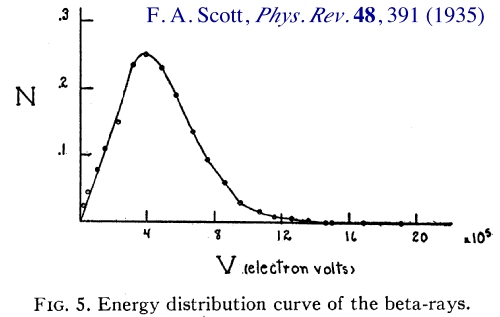
\includegraphics[width=0.5\textwidth]{fig/weak/betaspectrum.jpg}
\caption{Energy spectrum of $\beta$ rays in Radium A. A continuous energy
  spectrum up to the $E_e^{\mathrm{2-body}}$ is observed.
 \label{fig:betaEnergySpectrum}}
\end{figure}
 However, in 1930
 \href{http://www.nobel.se/physics/laureates/1935/chadwick-bio.html}{James
 Chadwick} discovered that, for beta radiation, this is not
 true. Instead energy spectra like the one in
 \figref{fig:betaEnergySpectrum} are observed, covering the entire
 kinematic range between $zero$ and the energy one would expect for 2
 body decays according to \eqref{eq:twoBodyEnergy}. One rather
 unattractive explanation for this observation would be the violation
 of energy conservation.

\subsection{Neutrinos}

 To rescue Energy conservation, Pauli proposed in 1930 the existence
 of an additional particle, that would carry the missing energy in the
 decay. This particle would have to be
\begin{itemize}
 \item neutral to escape detection
 \item very light or massless, to account for observed endpoints of
 the electron energy spectra i.e. the observation some that electrons
 seem to carry so much energy away that they leave nothing for the
 neutrino, not even for it to sit there if it has mass.
 \item spin \half, to account for angular momentum conservation.
\end{itemize}
 Initially he called this particle ``neutron'', but after the
 discovery of the neutron by Chadwick, he followed a suggestion by
 Fermi and named it neutrino.

\subsection{Fermi's theory of nuclear reactions}

 The original description, that worked well up to a certain energy, was Fermi's 4-point reaction: Have a
 neutron as the ingoing particle, the (lighter) proton outgoing, and
 instead of a photon, emit an electron-neutrino \emph{pair}.
\\
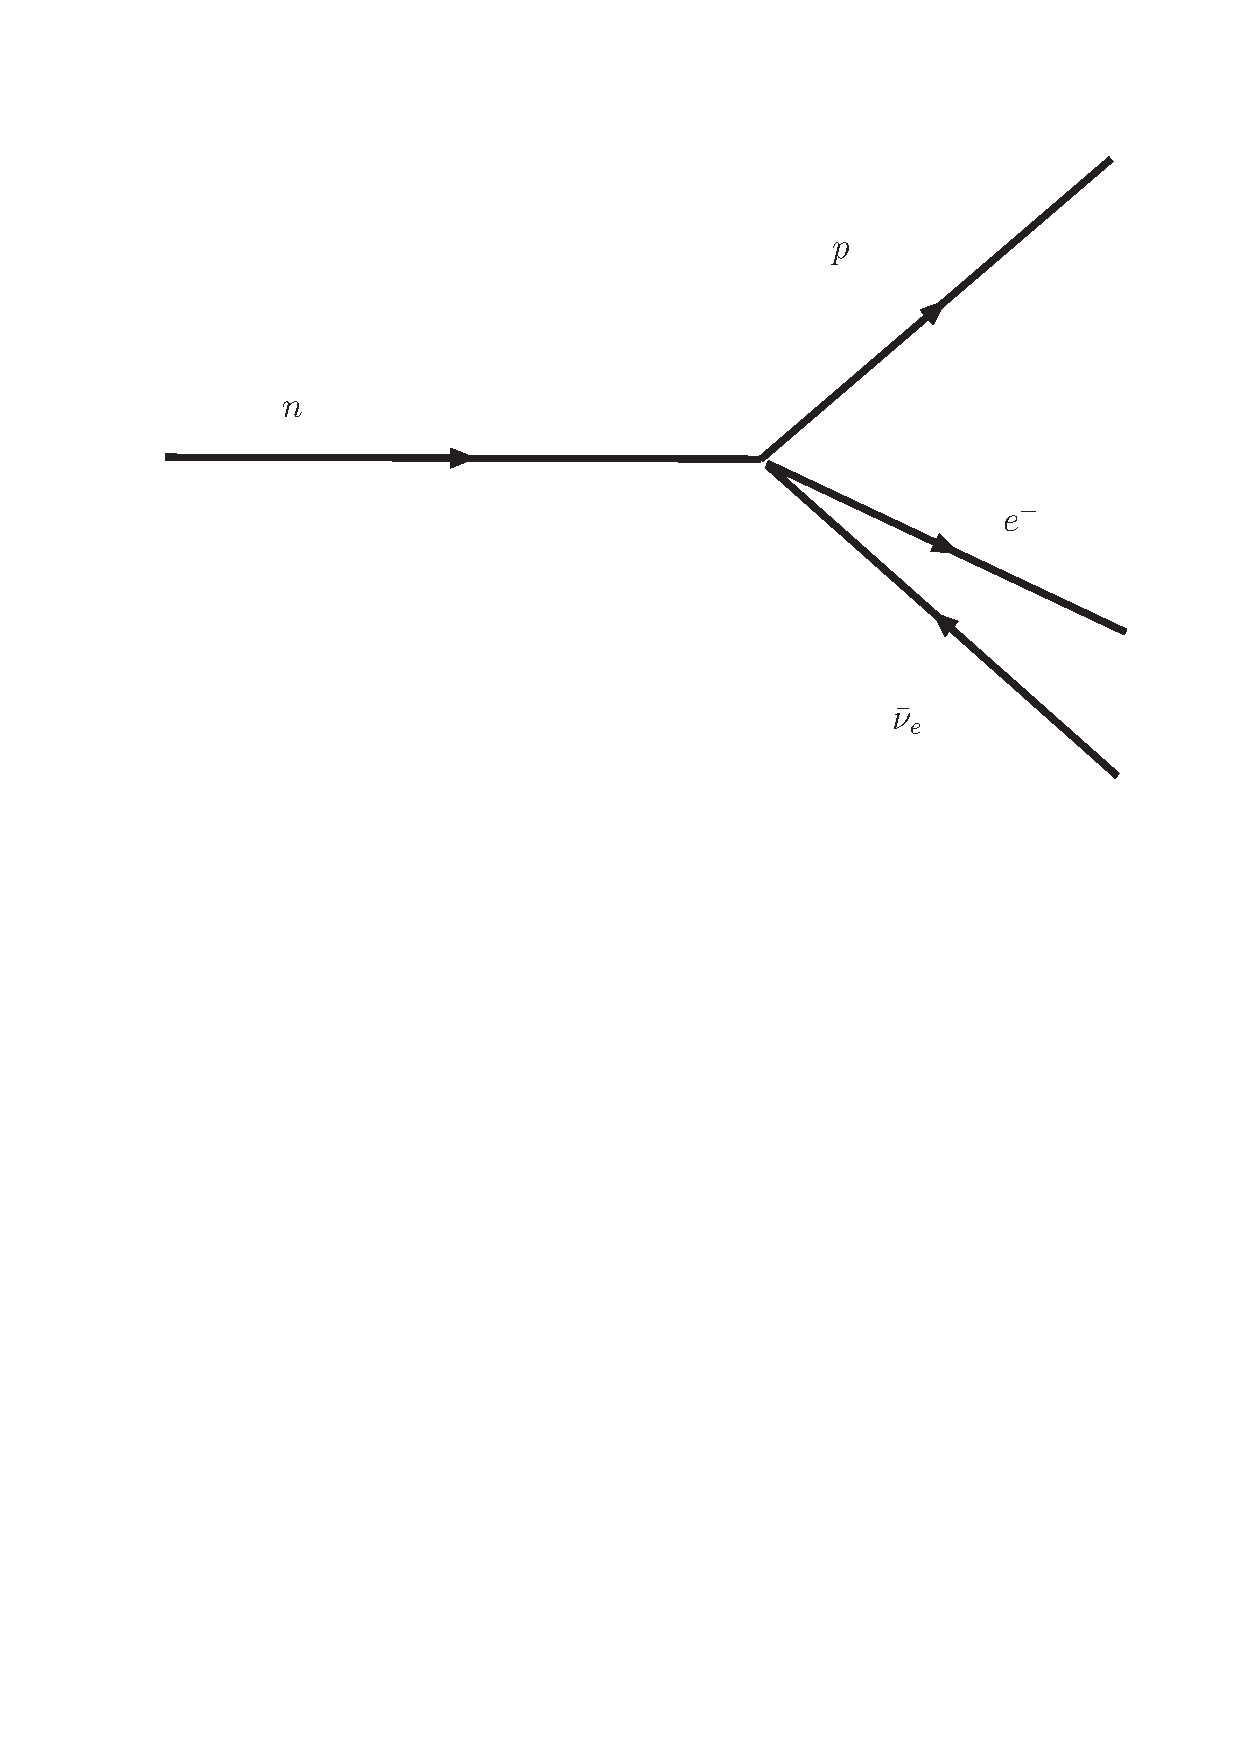
\includegraphics[width=0.5\textwidth]{fig/weak/fourPoing}
\\
The matrix elemement for that would simply be the vertex factor, which has a coupling strength of $\frac{G_F}{\sqrt{2}}$ ($G_F$ is known as "G-Fermi").

\subsection{Massive vector bosons}
Instead of a 4-point interaction, we describe this today as a $W$ exchange with vertex factor $g_w$. It leads to the same result as the Fermi fourpoint interaction for energies where $p^2 \ll M_W^2$ if we put $\frac{G_F}{\sqrt{2}} = \frac{g_W^2}{M_W^2}$. At energies with $p^2 \gg M_W^2$, we can neglect the $W$ mass and we get the same kind of behaviour as for a photon, however, with the electroweak coupling constant $g$ (which is actually larger than that of the photon). It's obvious that something will go wrong at $p^2 = M_W^2$, this can be avoided by changing the propagator to $\frac{1}{p^2 - M_W^2 + iM_W\Gamma_W}$ where $\Gamma_W$ represents the width of the $W$. We can usually leave it out since this is much smaller than $M_W$.
It's worth noting that people had identified strong theoretical reasons why the four-point interaction had to be modified before energies where it breaks down could be explored. 

\subsection{At this point, not all weak interactions were (yet) the same}
In fact, the picture above is a bit too simple. It was found that there are three different coupling constants. One for lepton vertices, that we call $g_W$ above and that applies to $e \nu_{e} W$, $\mu \nu_{\mu} W$, $\tau \nu_{\tau}W$ (although the $\tau$ was discovered later), one for the $ud W$ vertex (which is nearly $g_W$, but not quite) and one for the $usW$ vertex, which is much smaller.
Cabibbo had an ingenious idea how these three coupling constants could be unified. This described in the next section.
